\begin{sddsprog}{sddscontour}
  \item \textbf{description:}
  \verb|sddscontour| makes contour and color-map plots from an SDDS data set column, array data, or from a \verb|rpn| expression
  in terms of the values in the columns of a data set. It supports FFT interpolation and filtering and also provides
  \verb|-columnmatch| and waterfall modes for plotting multiple columns or pages. With the \verb|-3d| option, it
  can display the data as an interactive three-dimensional surface or bar plot that can be rotated with the mouse.
  If the data set contains more than one data page, data from successive pages is plotted on separate pages. This mode
  requires the Qt device.

  \item \textbf{examples:}
    Generate a two-dimensional color-shaded map of the function ${\rm sin(4\pi (x^2 + y^2))}$ on the region x:[-1, 1] and y:[-1, 1]:
    \begin{verbatim}
sddscongen example.sdds -xRange=-1,1,101 -yRange=-1,1,101 -zEquation="x x * y y * + 4 * pi * sin"
sddscontour example.sdds -scales=0,1,0,1 -shade
    \end{verbatim}
    \centerline{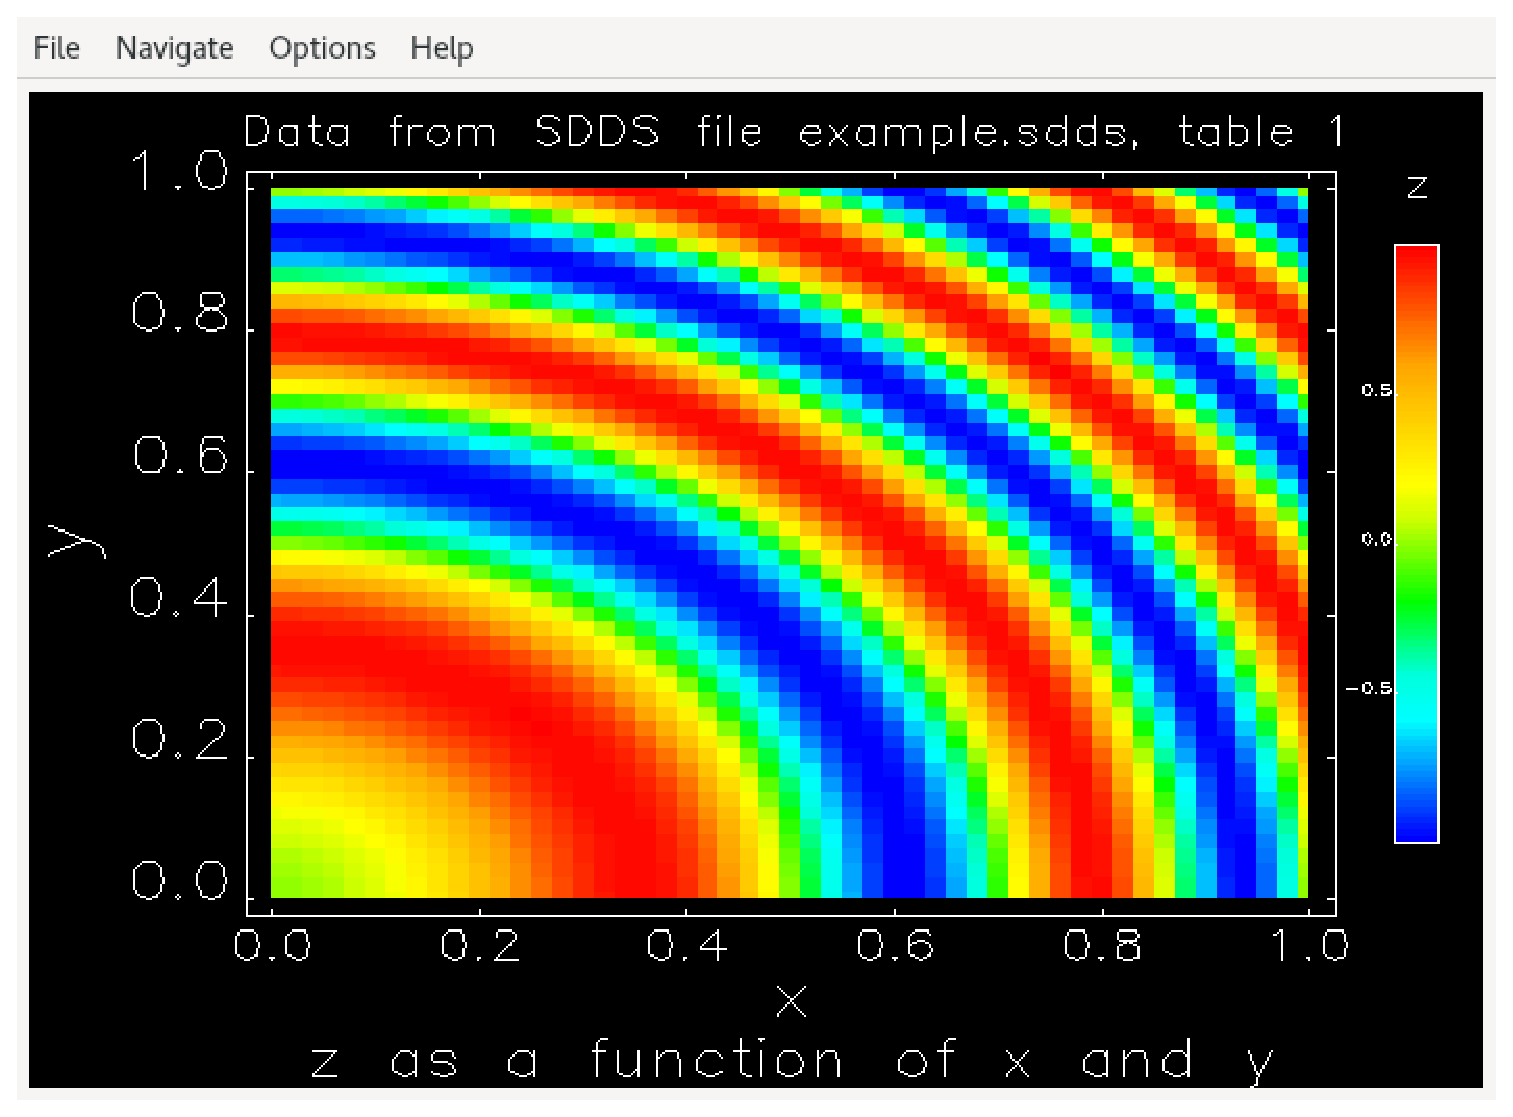
\includegraphics[width=3in]{2D-shade-plot.eps}}

    Generate a three-dimensional surface plot:
    \begin{verbatim}
sddscongen example.sdds -xRange=-1,1,101 -yRange=-1,1,101 -zEquation="x x * y y * + 4 * pi * sin"
sddscontour example.sdds -scales=0,1,0,1 -3d
    \end{verbatim}
    \centerline{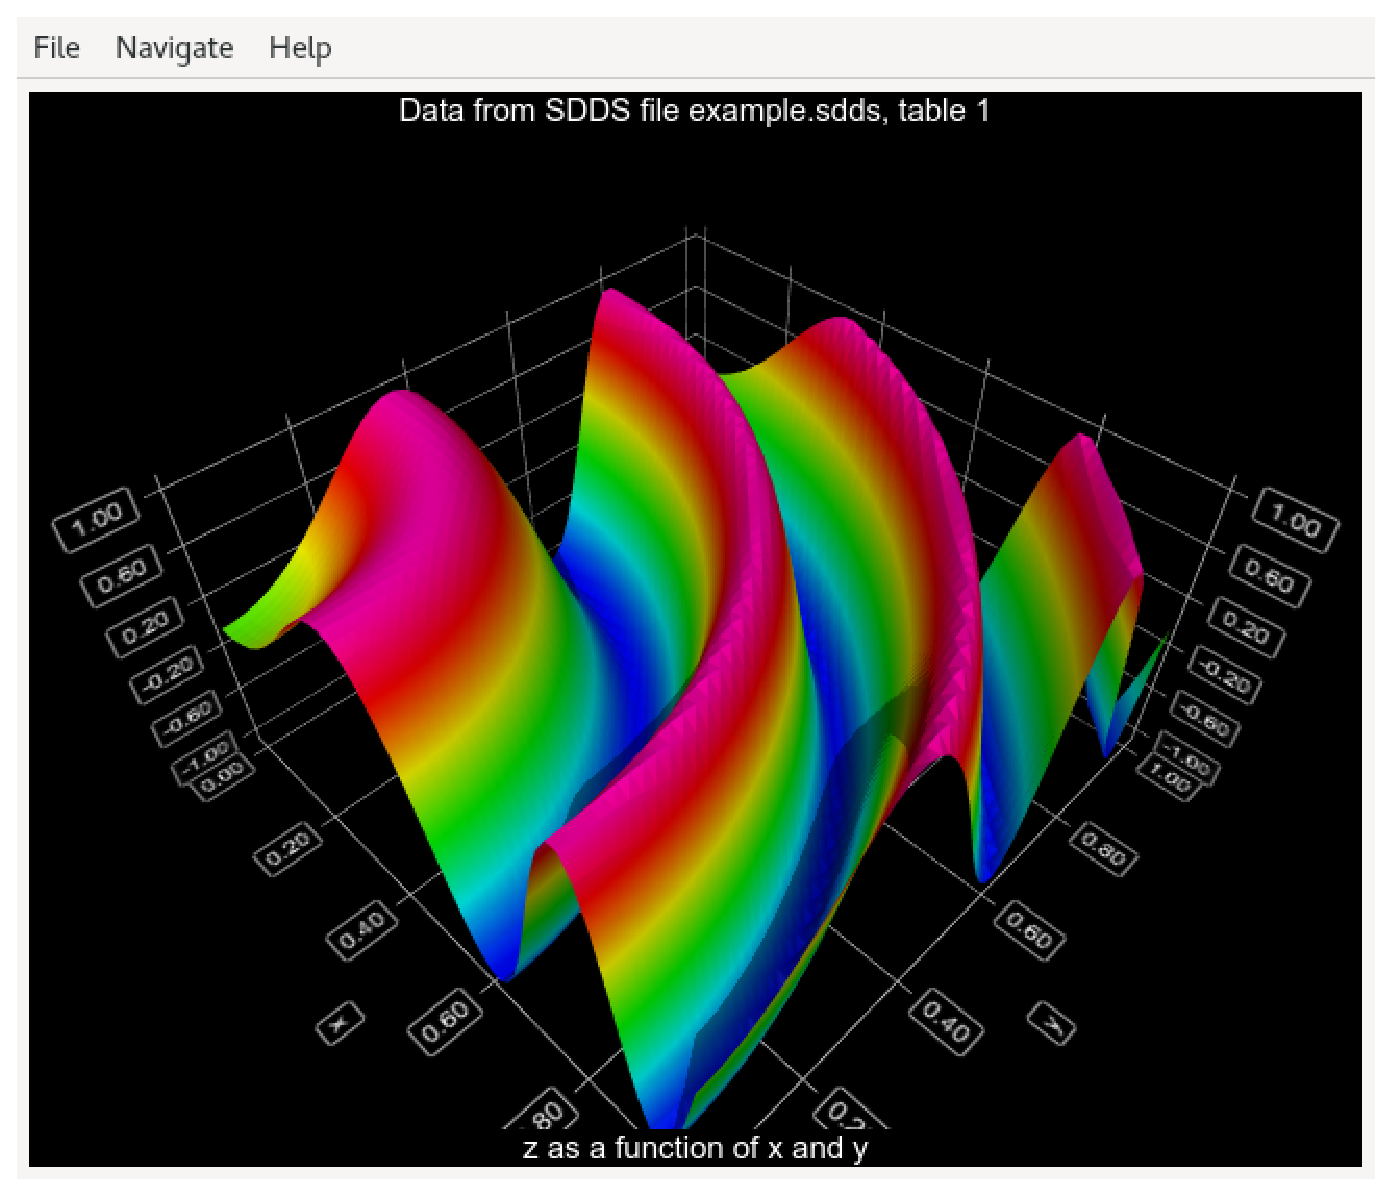
\includegraphics[width=3in]{3D-surface-plot.eps}}

    Toggle wireframe on with \verb|g|:
    \begin{verbatim}
sddscongen example.sdds -xRange=-1,1,101 -yRange=-1,1,101 -zEquation="x x * y y * + 4 * pi * sin"
sddscontour example.sdds -scales=0,1,0,1 -3d
# toggle wireframe on with 'g'
    \end{verbatim}
    \centerline{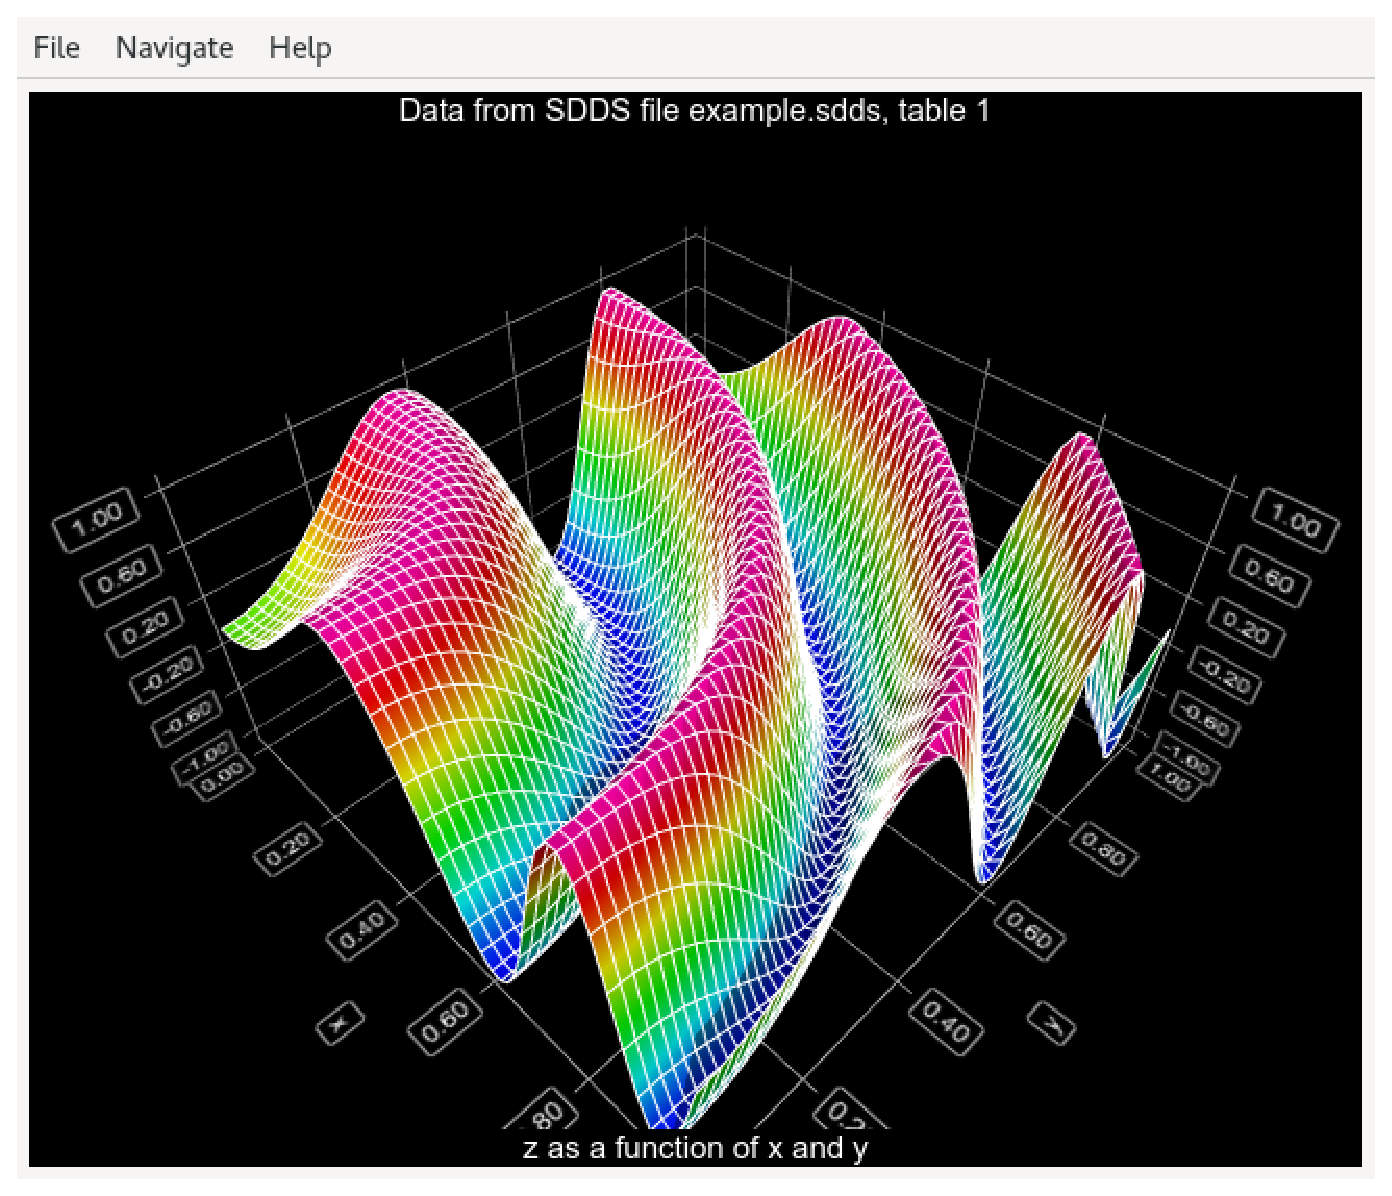
\includegraphics[width=3in]{3D-surface-plot2.eps}}

    Toggle wireframe on and surface off with \verb|g|:
    \begin{verbatim}
sddscongen example.sdds -xRange=-1,1,101 -yRange=-1,1,101 -zEquation="x x * y y * + 4 * pi * sin"
sddscontour example.sdds -scales=0,1,0,1 -3d
# toggle wireframe on and surface off with 'g'
    \end{verbatim}
    \centerline{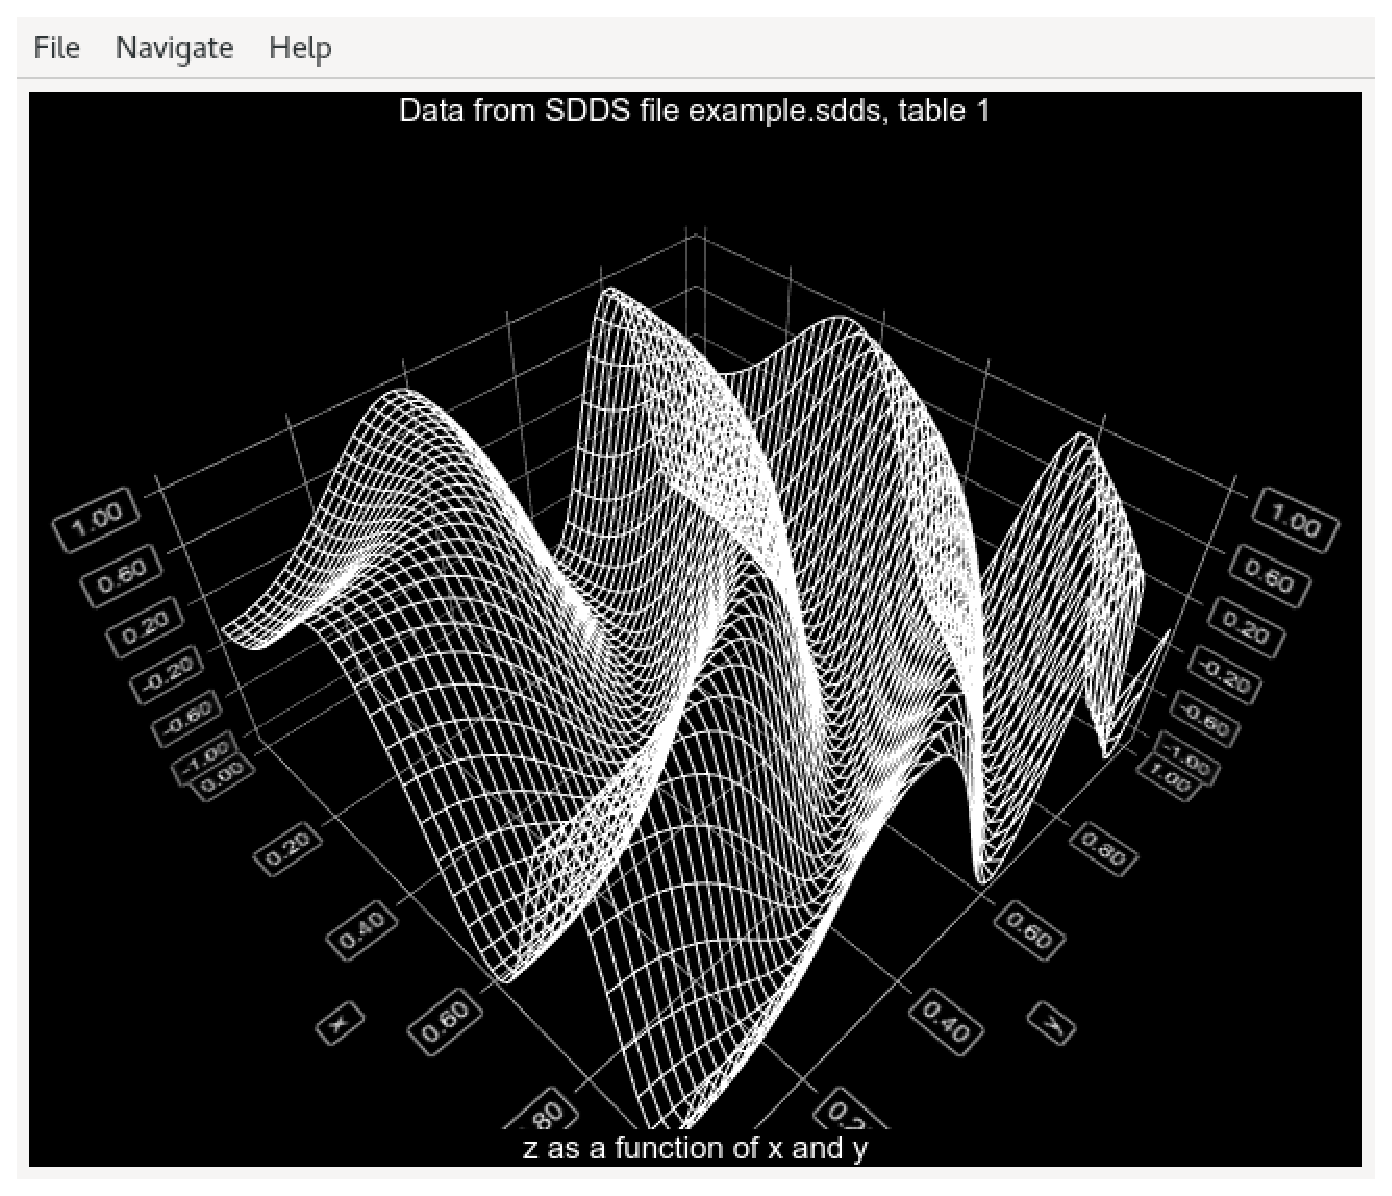
\includegraphics[width=3in]{3D-surface-plot3.eps}}

    Generate a three-dimensional bar plot:
    \begin{verbatim}
sddscongen example.sdds -xRange=-1,1,101 -yRange=-1,1,101 -zEquation="x x * y y * + 4 * pi * sin"
sddscontour example.sdds -scales=0,1,0,1 -3d=bar
    \end{verbatim}
    \centerline{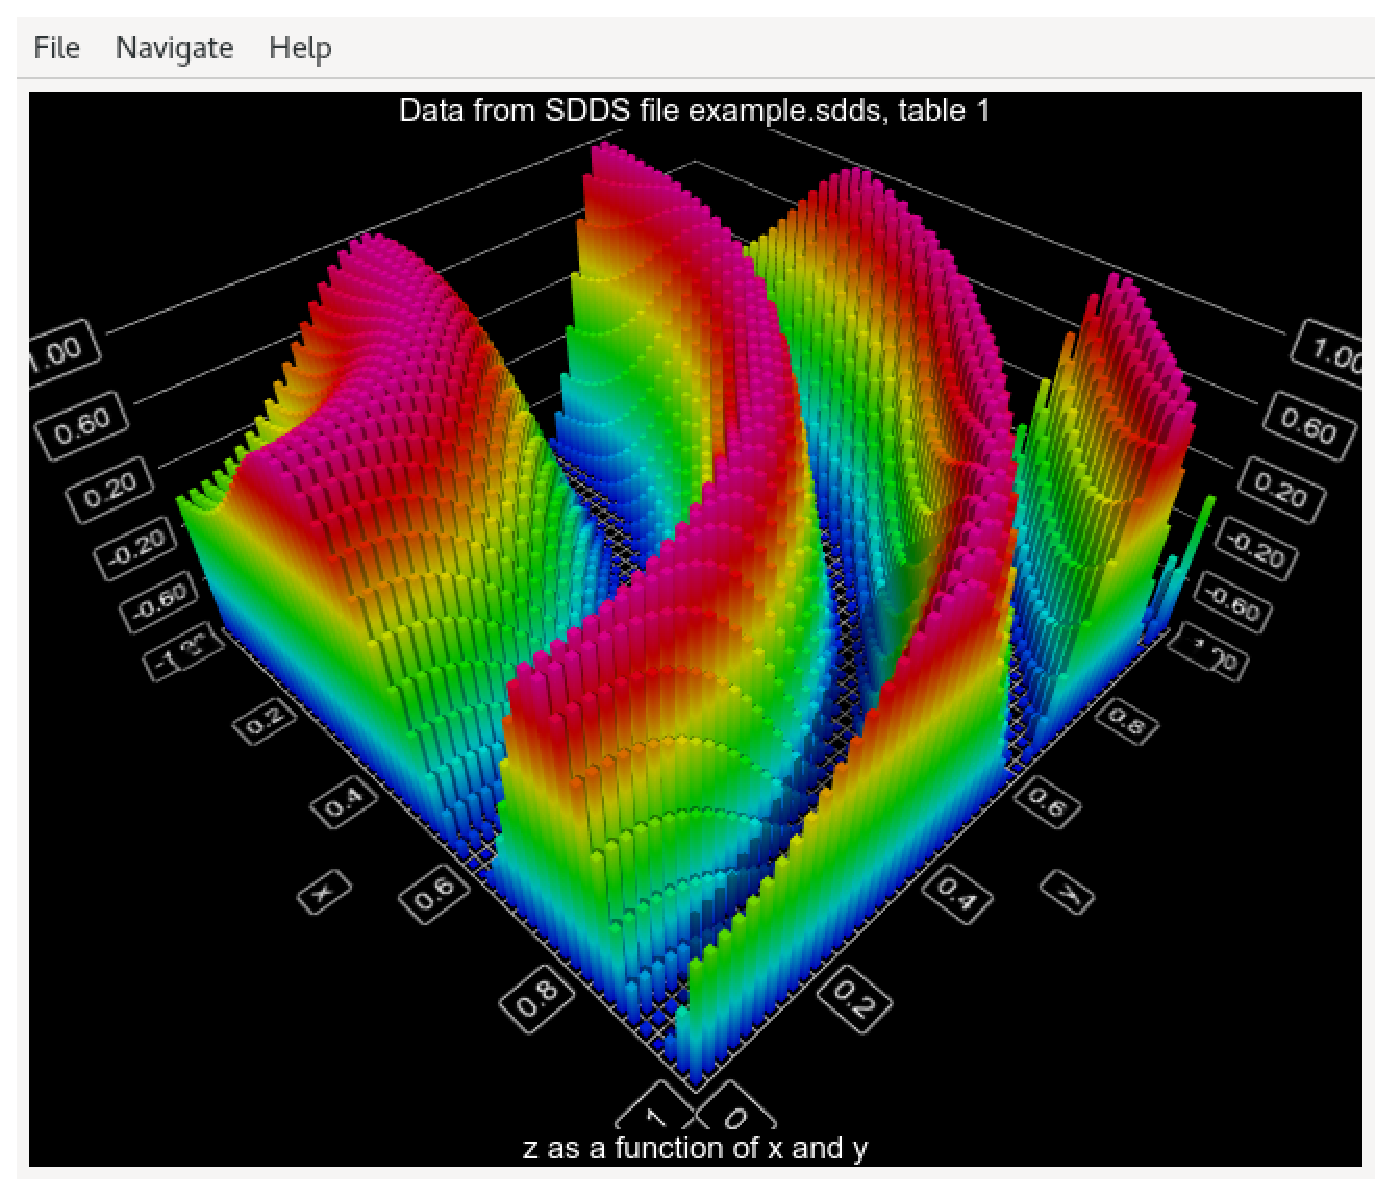
\includegraphics[width=3in]{3D-bar-plot.eps}}

    Generate a three-dimensional scatter plot:
    \begin{verbatim}
sddscongen example.sdds -xRange=-1,1,101 -yRange=-1,1,101 -zEquation="x x * y y * + 4 * pi * sin"
sddscontour example.sdds -scales=0,1,0,1 -3d=scatter
    \end{verbatim}
    \centerline{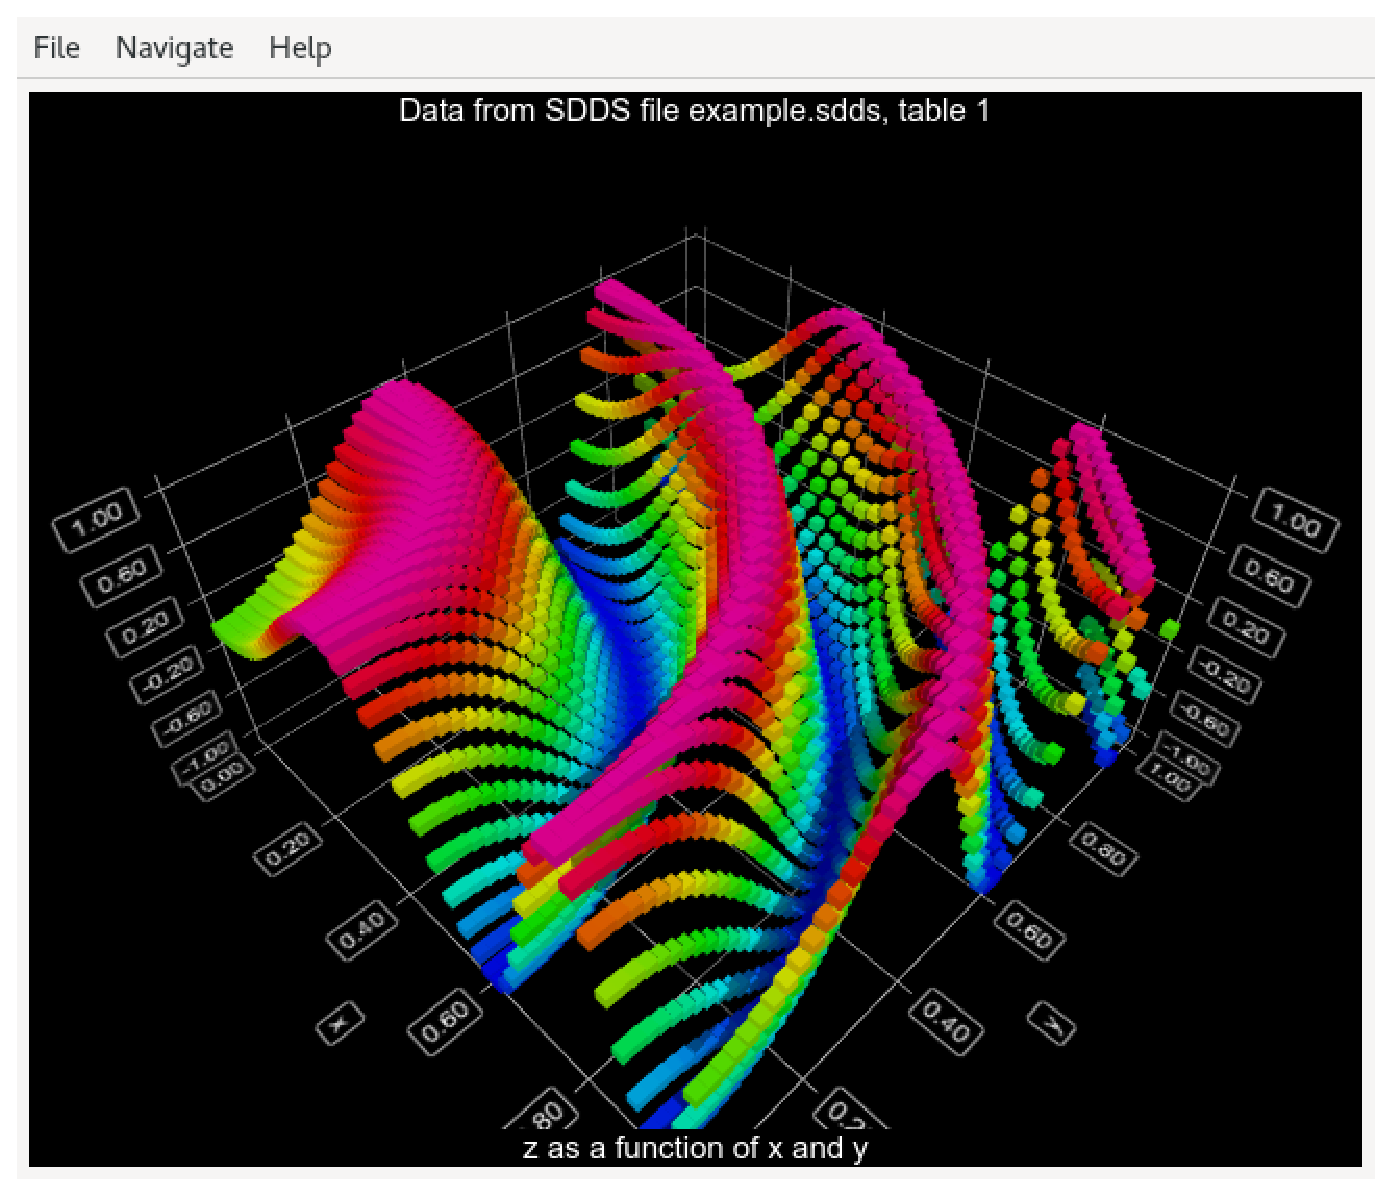
\includegraphics[width=3in]{3D-scatter-plot.eps}}

  \item \textbf{synopsis:}
  \begin{verbatim}
sddscontour [-pipe[=input][,output]] [<inputfile>] [options]
  \end{verbatim}
  \item \textbf{switches:}
    \begin{itemize}
    \item Choice of what to plot and data source:
\begin{flushleft}{\tt
[{ -quantity={\em columnName} | -equation={\em rpnExpression}[,algebraic] |
  -columnmatch={\em indepColumnName},{\em matchingExpression}} |
 -waterfall=parameter=<parameter>,independentColumn=<xColumn>,
             colorColumn=<colorColumn>[,scroll=vertical|horizontal]]
[-array=<zArray>[,<xArray>,<yArray>]] [-swaparray]
[-xyz={\em xColumnName},{\em yColumnName},{\em zColumnName}]
[-3d[=surface|bar|scatter]]
}\end{flushleft}
\begin{itemize}
        \item \verb|quantity| --- Specifies the name of the column to make a contour or color map of.
        \item \verb|equation| --- Specifies a \verb|rpn| expression to make a contour or color map of.
        The expression may refer to the values in the columns by the appropriate column name, and may
        also refer to the variable values by name.  Adding \verb|algebraic| allows the
        expression to be given in standard algebraic form instead of RPN.
        \item \verb|columnmatch| --- Specifies plotting of all columns matching {\em matchingExpression}
        as a function of the column {\em indepColumnName}.  Each matching column is displayed as a horizontal
        color bar.
        \item \verb|waterfall| --- Specifies plotting of {\em colorColumn} in all pages as a function of the
        {\em independentColumn}. The {\em parameter} in each page is displayed as horizontal or vertical (provided
        by the {\em scroll}) bar, the default is horizontal. The {\em independentColumn} should be the same in
        each page.
        \item \verb|array| --- Reads data from an SDDS array named {\em zArray}.  Optional one-dimensional arrays
          {\em xArray} and {\em yArray} may be given for axis values.
        \item \verb|swaparray| --- Requests that the row and column order of array data be swapped.
        \item \verb|xyz| --- Specifies the names of two independent columns {\em xColumnName} and {\em yColumnName}, along with
          a third dependent column {\em zColumnName} that is plotted as a function of the others.
          The x and y values must form a grid.
        \item \verb|-3d| --- Displays the data as an interactive 3-dimensional surface (\verb|-3d| or \verb|-3d=surface|), bar plot (\verb|-3d=bar|), or scatter plot (\verb|-3d=scatter|) that can be rotated with the mouse. Requires the Qt device.
        \end{itemize}

        In the case of the first two choices, the file must contain
tabular data with at least one numeric column, which will be organized
into a 2d array with R rows and C columns.  By default, the values are
assumed to come in row-major order (i.e., the file should contain a
series of R sequences each containing the C values of a single row).
The parameters of the 2d grid over which the plot is to be made are
communicated to the program in one of two ways:

\begin{enumerate}

\item The string parameters \verb|Variable1Name| and \verb|Variable2Name| contain the names of the
x and y axis variables, which I'll represent as {\em x} and {\em y} respectively.  The program expects to find
six more parameters, with names {\em x}\verb|Minimum|, {\em x}\verb|Interval|, and {\em x}\verb|Dimension|,
and similarly for {\em y}.  These parameters must be numeric, and contain the minimum value, the interval
between grid points, and the number of points, respectively, for the dimension in question.
The data must be arranged so that {\em y} varies fastest as the row in the file increases.  Put another
way, variable 1 is the row index and variable 2 is the column index.
\item The numeric parameters \verb|NumberOfRows| and \verb|NumberOfColumns| contain the values of R and
C, respectively.
\end{enumerate}
Use \verb|-v1v2preferred| to force the first method to be used when both parameter sets are present.

    \item \verb|rpn| control:
\begin{flushleft}{\tt
[-rpndefinitionsfiles={\em filename}[,{\em filename}...]]
[-rpnexpressions={\em setupExpression}[,{\em setupExpression}...][,algebraic]]
[-rpntransform={\em expression}[,algebraic]]
}\end{flushleft}
        \begin{itemize}
        \item \verb|rpndefinitionsfiles| --- Specifies the names of files containing \verb|rpn| expressions
        to be executed before any other processing takes place.
        \item \verb|rpnexpressions| --- Specifies \verb|rpn| expressions to be executed before any other processing
         takes place, immediately after any definitions files.  Adding \verb|algebraic| treats the
         expressions as standard algebraic formulas.
        \item \verb|rpntransform| --- Specifies an \verb|rpn| expression applied to each data value after it is read.
         Use \verb|algebraic| to supply the transform in algebraic form.
        \end{itemize}
    \item Data range control:
\begin{flushleft}{\tt
[-fixedrange] [-showgaps]
}\end{flushleft}
        \begin{itemize}
        \item \verb|fixedrange| --- Retains the initial data range for all pages, rather than recomputing it.
        \item \verb|showgaps| --- Leaves regions with missing data unplotted rather than interpolated.
        \end{itemize}
    \item Shade and contour control:
\begin{flushleft}{\tt
\{-shade={\em number}[,{\em min},{\em max},gray] | -contours={\em number}[,{\em min},{\em max}]\}
[-labelcontours={\em interval}[,{\em offset}]]
[-levellist={\em listOfLevels}] [-limitlevels={minimum=<value>,}{maximum=<value>}]
[-mapshade={\em hue0},{\em hue1}]
}\end{flushleft}
        \begin{itemize}
        \item \verb|shade| --- Specifies that a color (or grey-scale) map should be produced, with the
        indicated {\em number} of shades mapped onto the range from {\em min} to {\em max}.  If {\em min}
        and {\em max} are not given, they are taken to be equal to the minimum and maximum data values.
        \item \verb|contours| --- Specifies that contour lines should be drawn, with the
        indicated {\em number} of lines for the range from {\em min} to {\em max}.  If {\em min}
        and {\em max} are not given, they are taken to be equal to the minimum and maximum data values.
        \item \verb|labelcontours| --- Specifies that every {\em interval}$^{th}$ contour line, starting with
        the {\em offset}$^{th}$ line, should be labeled with the contour value.
        \item \verb|levellist| --- Gives an explicit comma-separated list of contour or shade levels to use.
        \item \verb|limitlevels| --- Restricts contour or shade levels to the specified range.
        \item \verb|mapshade| --- Maps the shades from hue {\em hue0} to {\em hue1} instead of the default rainbow.
        \end{itemize}
    \item Image processing:
\begin{flushleft}{\tt
[-interpolate={\em nx},{\em ny}[,{floor | ceiling | antiripple}]] [-filter={\em xcutoff},{\em ycutoff}]
}\end{flushleft}
        \begin{itemize}
        \item \verb|interpolate| --- Specifies that the 2d map should be interpolated to have {\em nx} times
        more rows (or x grid points) and {\em ny} times more columns (or y grid points).  Since FFTs are used to
        do the interpolation, the original number of grid points must be a power of 2, as must the factor.  Giving
        a factor of 1 disables interpolation for the dimension in question.  \verb|floor|, \verb|ceiling|,
        and \verb|antiripple| specify image processing of the interpolated map.  \verb|floor| and \verb|ceiling|
        respectively force values below (above) the minimum (maximum) value of the data to be set equal to that
        value.  \verb|antiripple| causes the map to be altered so that non-zero values in the new map between
        zero values on the original map are set to zero; this suppresses ripples that sometimes occur in regions
        where the data was originally all zero.
        \item \verb|filter| --- Applies low-pass filters to the data with the specified normalized cutoff
        frequencies.  The integer cutoff values give the number of frequencies starting at the Nyquist frequency
        that are to be eliminated.
        \end{itemize}
    \item Plot labeling:
\begin{flushleft}{\tt
[-xlabel={\em string|@<parameter-name>[,scale=<value>][,edit=<string>]}]
[-ylabel={\em string|@<parameter-name>[,scale=<value>][,edit=<string>]}]
[-title={\em string|@<parameter-name>|filename[,edit=<string>]}]
[-topline={\em string|@<parameter-name>|filename[,edit=<string>][,format=<string>]}]
[-toptitle] [-nolabels] [-noscales] [-noborder] [-datestamp]
[-fixfontsize[=all=.02][,legend=.015][,<x|y>xlabel=<value>][,<x|y>ticks=<value>][,title=<value>][,topline=<value>]]
}\end{flushleft}
        \begin{itemize}
        \item \verb|xlabel|, \verb|ylabel|, \verb|title|, \verb|topline| --- These specify strings to be placed
                in the various label locations on the plot. If @<parameter-name> is provided, the value of the
                given parameter will be printed.  If {\em -topline=filename[,edit=<string>][,format=<string>]} or
                {\em -title=filename[,edit=<string>]} option is provided, then the input file name or edited file
                name (if edit command is also provided) will be printed to the topline or title.  The
                \verb|format| qualifier allows a printf-style format for numeric parameter values in the topline.
        \item \verb|toptitle| --- Requests that the title label be placed at the top of the plot, rather than
                at the bottom.
        \item \verb|nolabels| --- Requests that no labels be placed on the plot.
        \item \verb|noscales| --- Requests omission of the numeric scales.
        \item \verb|noborder| --- Requests omission of the border around the data.  Implies \verb|-noscales|.
        \item \verb|datestamp| --- Requests that the date and time be placed on the plot.
        \item \verb|fixfontsize| --- Disables automatic font scaling and sets the font sizes explicitly.
        \end{itemize}
    \item Plot tick labeling (only valid for -columnmatch plots):
\begin{flushleft}{\tt
[-xrange=minimum={\em value}|@{\em parameterName},maximum={\em value}|@{\em parameterName}]
[-yrange=minimum={\em value}|@{\em parameterName},maximum={\em value}|@{\em parameterName}]
[-xaxis=scaleValue=<value>|scaleParameter=<name>[,offsetValue=<number>|offsetParameter=<name>]]
[-yaxis=scaleValue=<value>|scaleParameter=<name>[,offsetValue=<number>|offsetParameter=<name>]]
[-ystrings=[edit=<editCommand>][,sparse=<integer>][,scale=<value>]]
[-yeditstrings=<editCommand>]
}\end{flushleft}
        \begin{itemize}
        \item \verb|xrange| --- Specifies the minimum and maximum value of the x axis. The value can be provided or obtained from parameters.
                If \verb|-xrange| is provided, the independent column will be ignored.
        \item \verb|yrange| --- Specifies the minimum and maximum value of the y axis. The value can be provided or obtained from parameters.
                If \verb|-yrange| is provided, the y tick labels will be numerically labeled with the provided range.
        \item \verb|xaxis| --- Sets scale and offset for x-axis tick labels using explicit values or parameter references. Labels are computed as \verb|index * scale + offset|.
        \item \verb|yaxis| --- Sets scale and offset for y-axis tick labels using explicit values or parameter references. Labels are computed as \verb|index * scale + offset|.
        \item \verb|ystrings| --- Controls the y tick labels, allowing optional editing, sparsity, and scaling.
        \item \verb|yeditstrings| --- Provides an edit command for y tick labels; equivalent to using \verb|edit| with \verb|-ystrings|.
        \end{itemize}
        {\bf For example}, parameters {\em origin1}, {\em delta1}, {\em max\_ext1}, {\em origin2}, {\em delta2}, and {\em max\_ext2} in \href{https://ops.aps.anl.gov/manuals/example_files/sddscontour.input1}{sddscontour.input1} define the coordinate ranges.
        The first three give the minimum, spacing, and maximum of the x coordinate, while the latter three give the same for y.
        The {\em Index} column provides the x index so that {\em x = Index * delta1 + origin1}.  Columns {\em Ex_n} contain field
        values at {\em y = (n-1)*delta2 + origin2}.  Without \verb|-xrange| and \verb|-yrange| the plot shows index values rather
        than coordinates:
        \begin{flushleft}{\tt \bf
            sddscontour sddscontour.input1 -columnmatch=Index,Ex* -ystrings=sparse=10 -ylabel=y -shade
            \href{https://ops.aps.anl.gov/manuals/example_files/sddscontour1_img.html}{show\_plot}
        }\end{flushleft}

        To remove the string portion of the y tick labels, use \verb|-ystrings|:
        \begin{flushleft}{\tt \bf
            sddscontour sddscontour.input1 -columnmatch=Index,Ex* -ystrings=edit=\%/Ex_//,sparse=10 -ylabel=y -shade
            \href{https://ops.aps.anl.gov/manuals/example_files/sddscontour2_img.html}{show\_plot}
        }\end{flushleft}

        The previous plot still labels y with indexes.  Supplying \verb|-yrange| displays the actual y values:
        \begin{flushleft}{\tt \bf
            sddscontour sddscontour.input1 -columnmatch=Index,Ex* -yrange=minimum=@origin2,maximum=@max\_ext2 -ylabel=y -shade
            \href{https://ops.aps.anl.gov/manuals/example_files/sddscontour3_img.html}{show\_plot}
        }\end{flushleft}

        To label the x axis with coordinate values, add \verb|-xrange|:
        \begin{flushleft}{\tt \bf
            sddscontour sddscontour.input1 -columnmatch=Index,Ex* -yrange=minimum=@origin2,maximum=@max\_ext2 -xrange=minimum=@origin1,maximum=@max\_ext1 -xlabel=x -ylabel=y -shade \href{https://ops.aps.anl.gov/manuals/example_files/sddscontour4_img.html}{show\_plot}
        }\end{flushleft}

        In this case the independent column ({\em Index}) is redundant.  The \verb|-xrange| option allows contour plots of a set
        of columns without an explicit independent column.  If \verb|sddsprocess| is used to create an x column via
        {\em x=Index * delta1 + origin1}, the same plot results from
        \begin{flushleft}{\tt \bf
            sddscontour sddscontour.input1 -columnmatch=x,Ex* -yrange=minimum=@origin2,maximum=@max\_ext2 -ylabel=y -shade \href{https://ops.aps.anl.gov/manuals/example_files/sddscontour5_img.html}{show\_plot}
        }\end{flushleft}

        These examples obtain \verb|xrange| and \verb|yrange| from parameters, but fixed values may also be given on the command line.


    \item Data scaling:
\begin{flushleft}{\tt
[-deltas[=\{fractional | normalize\}]] [-logscale[={\em floor}]] [-xlog]
}\end{flushleft}
        \begin{itemize}
        \item \verb|deltas| --- For use with \verb|-columnmatch| and \verb|-waterfall| option.  Specifies plotting
        only differential values (relative to the mean of each column).  If the \verb|fractional|
        qualifier is given, then the differential values normalized to the individual
        means are plotted.  If the \verb|normalize| qualifier is given, then all differential values
        are normalized to the range [-1, 1] before plotting.
        \item \verb|logscale| --- Specifies plotting the base-10 logarithm of the values.  If a
        {\em floor} value is given, it is added to each value prior to taking the logarithm; this
        can help prevent taking the log of zero, for example.
        \item \verb|xlog| --- Plots the horizontal coordinate using a base-10 logarithmic scale.
        \end{itemize}
    \item Miscellaneous plot control:
\begin{flushleft}{\tt
[-scales={\em xl},{\em xh},{\em yl},{\em yh}]
[-swapxy] [-yflip] [-equalaspect[={-1,1}]]
[-layout={\em nx},{\em ny}] [-ticksettings={xy}time]
[-nocolorbar] [-thickness={\em integer}] [-fillscreen]
[-shapes={\em filename},{\em xColumn},{\em yColumn}[,type={\em lineType}][,thickness={\em value}]]
[-symbols={\em filename},{\em xColumn},{\em yColumn}[,type={\em symbolType}][,fill][,thickness={\em value}][,scale={\em factor}]]
[-drawline=\{x0value={\em value} | p0value={\em value} | x0parameter={\em name} | p0parameter={\em name}\},
            \{x1value={\em value} | p1value={\em value} | x1parameter={\em name} | p1parameter={\em name}\},
            \{y0value={\em value} | q0value={\em value} | y0parameter={\em name} | q0parameter={\em name}\},
            \{y1value={\em value} | q1value={\em value} | y1parameter={\em name} | q1parameter={\em name}\},
            [,linetype={\em integer}][,thickness={\em integer}][,clip]]
}\end{flushleft}
        \begin{itemize}
        \item \verb|scales| --- Specifies the extent of the plot region.
        \item \verb|swapxy| --- Requests that the horizontal and vertical coordinates be interchanged.
        \item \verb|yflip| --- Reverses the vertical direction of the plot.
        \item \verb|equalaspect| --- Requests plotting with an aspect ratio of 1.  If the '1' qualifier
        is given, then the aspect ratio is achieved by changing the size of the plot region within the window;
        this is the default.
        If the '-1' qualifier is given, then the aspect ratio is achieved by changing the size of the plot region
        in user's coordinates.
        \item \verb|layout| --- Specifies that each page of the plot should have a {\em nx} by {\em ny} grid of contour plots.
        \item \verb|ticksettings| --- Specify use of time mode for tick settings.
        \item \verb|nocolorbar| --- Specify suppression of the color bar in \verb|-shade| mode.
        \item \verb|thickness| --- Sets the line thickness used for drawing.
        \item \verb|fillscreen| --- Expands the plot to fill the entire screen.
        \item \verb|shapes| --- Plots line shapes read from {\em filename} using columns {\em xColumn} and {\em yColumn}.
        \item \verb|symbols| --- Plots symbols from {\em filename} using columns {\em xColumn} and {\em yColumn}.
        \item \verb|drawline| --- Requests drawing of lines on the plot, using any combination of real coordinate values
          or plot-space values, either specified as literal values or drawn from parameters in the data file.
          Optional qualifiers \verb|linetype|, \verb|thickness|, and \verb|clip| control the appearance and clipping of
          the line. Suitable for multi-page files.
        \end{itemize}
    \item Miscellaneous:
\begin{flushleft}{\tt
[-pipe] [-device={\em name}[,{\em deviceArguments}]]
[-output={\em filename}] [-verbosity[=level]]
[-convertunits={column|parameter},<name>,<new-units-name>,<old-units-name>[,<factor>]]
}\end{flushleft}
        \begin{itemize}
        \item \verb|pipe| --- Reads from the standard input and/or writes to the standard output.
        \item \verb|device| --- Specifies the device name and optional device-specific arguments. Qt device
        arguments include \verb|-dashes <0|1>|, \verb|-linetype <filename>|, \verb|-movie 1| [\verb|-interval <sec>|],
        \verb|-keep <number>|, \verb|-share <name>|, \verb|-timeoutHours <hours>|, and \verb|-spectrum|. png devices
        take rootname and template identifiers. {\tt rootname={\em string}} specifies a rootname
        for automatic filename generation; the resulting filenames are of the form {\em rootname}.DDD, where DDD
        is a three-digit integer. {\tt template={\em string}} provides a more general facility; one uses it to
        specify an sprintf-style format string to use in creating filenames. For example, the behavior obtained
        using {\tt rootname={\em name}} may be obtained  using {\tt template={\em name}.\%03ld}.
        \item \verb|output| --- Requests SDDS output of a new file containing the data with any modifications
                resulting in the processing requested.
        \item \verb|verbosity| --- Sets the verbosity level of informational printouts. Higher integer values
                of the \verb|level| parameter result in more output.
        \item \verb|convertunits| --- Converts the units of a named column or parameter to new units, applying an optional factor.
        \end{itemize}
    \end{itemize}
  \item \textbf{see also:}
    \begin{itemize}
      \item \progref{sddscongen}
      \item \progref{sddshist2d}
      \item \progref{sddsimageconvert}
      \item \progref{sddsimageprofiles}
      \item \progref{sddsplot}
      \item \progref{sddsspotanalysis}
      \item \progref{rpn}
    \end{itemize}
  \item \textbf{author:} M. Borland, ANL/APS.
\end{sddsprog}
